\documentclass{cslthse-msc}
\usepackage[utf8]{inputenc}
\usepackage[english]{babel}
\usepackage{amsmath}
\usepackage{amsfonts}
\usepackage{amssymb}
\usepackage{amsthm}
%\usepackage{makeidx}
\usepackage{graphicx}
\usepackage{algpseudocode}
\usepackage[titletoc, header, page]{appendix}

\usepackage{hyperref}

\newtheorem{definition}{Definition}[chapter]

%\geometry{showframe}

\author{
	Philip Ståhl \\
	{\normalsize \href{mailto:ada10pst@student.lu.se}{\texttt{ada10pst@student.lu.se}}}
	\and
	Jonatan Broberg \\
    {\normalsize \href{mailto:elt11jbr@student.lu.se
}{\texttt{elt11jbr@student.lu.se}}}
}

\title{Dynamic Fault-Tolerance and Task Scheduling in Distributed Systems}
\subtitle{}
\company{Mobile and Pervasive Computing Institute (MAPCI), Lund University}
\supervisors{Björn Landfeldt, \href{mailto:bjorn.landfeldt@eit.lth.se}{\texttt{bjorn.landfeldt@eit.lth.se}}}{}
\examiner{Christian Nyberg, \href{mailto:christian.nyberg@eit.lth.se}{\texttt{christian.nyberg@eit.lth.se}}}

\date{\today}
%\date{January 16, 2015}

\acknowledgements{
If you want to thank people, do it here, on a separate right-hand page. Both the U.S. \textit{acknowledgments} and the British \textit{acknowledgements} spellings are acceptable.

We would like to thank MAPCI and our supervisor Björn Landfeldt for there input. % Maybe Ericsson as well!
Shub...something for input. 
We also would like to thank our examiner Christian Nyberg.
}

\theabstract{
This document describes the Master's Thesis format for the theses carried out at 
the Department of Computer Science, Lund University. 

Your abstract should capture, in English, the whole thesis with focus on the problem and solution in 150 words. It should be placed on a separate right-hand page, with an additional \textit{1cm} margin on both left and right. Avoid acronyms, footnotes, and references in the abstract if possible.

Leave a \textit{2cm} vertical space after the abstract and provide a few keywords relevant for your report. Use five to six words, of which at most two should be from the title.
}

\keywords{MSc, template, report, style, structure}

%% Only used to display font sizes
\makeatletter
\newcommand\thefontsize[1]{{#1 \f@size pt\par}}
\makeatother
%%%%%%%%%%


\begin{document}
\makefrontmatter

\chapter{Introduction} \label{ch:introduction} 
\section{Background and Motivation} 
Ensuring a certain level of reliability is of major concern for many cloud system providers. As cloud computing is growing rapidly and users are demanding more services and higher performance, load balancing and task scheduling in the cloud has become a very important and interesting research area. 
% Five -nine means less than 5 min and 15 seconds downtime/year, i.e. operational 99,999 % of the time
Cloud systems often consists of heterogeneous hardware and  ensuring a certain level of reliability is therefore a complex task as any of the components may fail at any time. 
\\\\
Guaranteeing properties such as high reliability, raises complexity to the resource allocation decisions, and fault-tolerance mechanisms in highly dynamic distributed systems. For cloud service providers, it is necessary that this increased complexity is taken care of without putting extra burden on the user. The system should therefore ensure these properties in a seamless way.
\\\\
As computational work is distributed across multiple resources, the overall reliability of the application decreases. To cope with this issue, a fault-tolerant design or error handling mechanism need to be in place. This is of particular interest for cloud service providers, as users often desire a certain level of reliability. In some cases, vendors, for example carrier providers, are obliged by law to achieve a certain level of availability or reliability. In these cases, one may need to sacrifice other quality aspects such as latency and resource usage. By using static and dynamic analysis of the infrastructure and the mean-time-between-failure for the given resources, a statistical model can be used in order to verify  that the desired level is reached. However, such a model should be dynamic, as failure rates are likely to vary over time, for example due to high or low load on the system. This is of particular importance for long running applications when requiring a certain level of reliability. Dispite fulfilling the required level at the time of deployment, as the state of the system changes, the level may no longer be fulfilled. This speaks for a dyanmic model.
\\\\
Reliability can be increased by cloning application tasks, where all clones produce the same output. This allows for both increased redundancy and an easy way of detecting errors. If the execution of one clone stops, e.g. due to hardware or link failure, it can easily be detected at the receiver side which allows for a scheduling mechanism to find a proper location for a new clone. This allows for continuing execution of the application even in case failure. Seamlessly being able to continue the execution, without losing any data is of particular interest in data stream processing.
\\\\
Some of the drawbacks of replicating a task n times, is that the resources needed increases. With $n$ replicas, all performing the same computation on the same input, one need $n$ times as much resources, and since only the work of one task is needed, a lot of computational resources is thus wasted. Dynamic analysis of the system could help in determining on which resources one should assign the tasks to for optimal resource usage and load balancing. 


\section{Related work} \label{sec:related_work}
The interest in reliability in distributed systems has gain increased knowledge. Due to the uncertain heteregenous environment of cloud and grid systems, increasing reliability is a complex task [TODO]. %TODO add reference

A lot of scheduling techniques has been designed, aiming at maximizing reliability of jobs in distributed environments, under various constraints such as meeting task deadlines or minimizing execution time \cite{algoOptTimeMaxRel} \cite{optTaskAllocationForMaxRel} \cite{taskAllocation} \cite{taskAllocationSwarm} \cite{algoMaxRelEndToEndConstraint} \cite{algoMinExTime}  \cite{schedReplicas}. Maximizing reliability for these algorithms are a secondary concern, while meeting the constraints are the primary. Other algorithms have been developed which put greater focus on increasing the reliability {\cite{optResourceAllMaxPerformance} \cite{matchSchedAlgoMinFailure}, and some have increased reliability as the primary objective \cite{safetyRelTaskAllocation} \cite{improvedTaskAllMaxRel}. Common for these scheduling techniques are that while they try to maximize reliability, they do not ensure a certain level of reliability to the user. Furthermore, the algorithms are usually static in the way that they do not account for the dynamic behaviour of distirbuted system, and they make assumptions such as known execution times of tasks.

A lot of work has been done in the area of designing fault-tolerant systems by using checkpoint/restart techniques [TODO]. %TODO add reference

Some attempts at designing fault-tolerant systems by the use of replication has been made \cite{designFaultTolerantSched}  \cite{evalReplicationSched} \cite{taskSchedulingReplication} \cite{effTaskReplMobGrid}. \cite{evalReplicationSched} assumes a static number of replicas, which is used for every application being deployed. Furthermore, they do not guarantee that all replicas are deployed, instead they use a best-effort approach, where replicas are deployed when resources are available. While both \cite{effTaskReplMobGrid}, \cite{taskSchedulingReplication} and \cite{designFaultTolerantSched} all dynamically determines the number of replicas based on the state of the system, it is static in the way thay failed replicas are not restarted. The reliability level for long running applications are therefore decreased if replicas fail.

%TODO
\cite{adaptiveCheckPointAndRep} proposes algorithms using checkpointing, replication, and a combination of both. One algorithm dynamically varies the number of replicas depending on system load. However, the algorithm reduces the number of replicas during peak hours, in order to reduce system load. Since the reliability of system decreases during higher load [TODO reference], one should increase the number of replicas to keep the desired level of reliability.

A fault-tolerant scheduling technique incorporates a replication scheme is presented in \cite{faultTolerantSchedPolicy}. While being dynamic in that failed replicas are restarted, it is static in that the user defines the number of replicas to use.

The techniques used in \cite{selfAdaptRel} \cite{dynAdaptRepl} are more dynamic and adaptive to the dynamic behaviour of distributed systems. However, reliability is defined as producing the correct result, and achieved by techniques like voting and \emph{k-modular redundancy}.



\iffalse %TODO start previous text
\newpage
PREVIOUS:
\\\\
A lot of work has been done in the area of designing fault-tolerant applications for distributed systems. Most of them use a checkpoint/restart based approach [X][TODO]. These techniques relies of the notion of a stable storage, such as a hard-drive, which is persistent even in the case of a system failure.
\\\\
To our knowledge, not much work has been done in dynamically ensuring a certain level of reliability through replication.\cite{effTaskReplMobGrid} aims at providing a certain level of fault-tolerance through replication in a Grid environment. They calculate the number of replicas based on the reliability of the grid resources. However, their approach is limited in that they use static replication, i.e. when a replica fails it is not replaced with a new one, no replicas are made during execution. Furthermore, they do not take the dynamic of the system into their failure model. While this may be sufficient for task with short execution times, it will be insufficient for long running tasks, as one or several replicas then are likely to die during the time of execution, and the reliability of the system vary over time, and thereby not fulfilling the level of fault-tolerance. Furthermore, the reliability model used is based on non-repairable objects, why they use a Weibull distribution of failures (?).
\\\\
Other work define reliability as producing the correct result \cite{selfAdaptRel} \cite{imprRelAdaptRL} \cite{X}. In these cases, reliability is achieved by various consensus algorithms, e.g. $k-modular redundancy$. The consensus problem can be viewed as a form of agreement. A consensus algorithm lets a task execute multiple times in parallel, independent of each other and afterwards they vote for which result is correct. This allows for detecting of Byzantine faults, i.e. when a node crashes or produce the incorrect result.
\\\\
A lot of work has been done focusing on reliability through scheduling techniques. \cite{SLASched} focus on meeting SLA by scheduling techniques, and while reliability can be part of an SLA, they focus on I/O performance and throughput. \cite{algoMaxRelEndToEndConstraint} focuses of maximizing reliability while still meeting end-to-end delay constraint, and \cite{algoMinExTime} and \cite{algoOptTimeMaxRel} both design algorithms aiming at minimizing time and cost while maximization of system reliability.
\\\\
Previous work usually assumes a constant failure rate \cite{algoMaxRelEndToEndConstraint} \cite{algoMinExTime} \cite{relModelDistSimSystem} \cite{optTaskAllocationForMaxRel} \cite{perfImplPerCheckPoint}. Such assumptions are unlikely to model the dynamicity of heterogeneous systems correctly. Therefore, we adapt a self-learning model, which adapts the failure rate for nodes in the system, and tries to avoid scheduling of tasks on unreliable nodes.
\\\\
There are a number of different redundancy alternatives, traditional redundancy executes an odd number of replicas and takes a vote for which result is correct. Progressive redundancy minimizes the number of replicas. Assume that with traditional redundancy $k \in {3,5,7...}$ replicas is executed, progressive redundancy only executes $(k+1)/2$ replicas and reaches consensus if all replicas return the same result. If consensus is not reached an additional number of replicas is executed until consensus is reached \cite{selfAdaptRel}. Furthermore there is an iterative redundancy alternative which focus is more on reaching a required level of reliability in comparison to reaching a level of consensus.
\\\\
\cite{selfAdaptRel} presents iterative redundancy and demonstrates that it is self-adapting. They say that the iterative redundancy self-adapts in three steps: (i) automatically detecting when a resource reliability drops and deploying more resources, (ii) by identifying unlucky parts of the computation and injecting extra redundancy and (iii) not relying on previous estimates of a resource reliability by making runtime resource allocations. Iterative redundancy calculates how many replicas is needed, executes them and check their result. If all results agree the task is done, otherwise the algorithm calculates the minimum number of addition jobs, deploys them and compare their result with the previous ones. The algorithm iterates this until the required level of reliability is met.
\\\\
A quite old but still relevant work is found in \cite{dynAdaptRepl} where they present a framework for dynamic replication with an adaptive control in an multi-agent system. They introduce the software architecture which can act as support for building reliable multi-agent systems. Since the available resources often are limited they say that it isn't feasible to replicate all components. Therefore they use a criticality for each agent which is allowed to evolve during runtime. The proposed solution allows for dynamically adapt the number of replicas and the replication strategy. The number of replicas is partly based on the agents critically and a predefined minimum number of replicas. From CPU usage time and communication activity an agent activity is calculated which is used in calculating the agents critically. One restriction they do in their fault model is that processes can only fail by permanent crashes.
\\\\
...Reliability evaluation?...
\\\\
MORE OR LESS COPIED:
\\\\
In this paper, we consider a heterogeneous DS that runs a hard real-time application (all the tasks should meet their deadlines). The goal is to find a task to processor assignment under which the overall reliability of the system (probability that all tasks run successfully) is maximized, while memory, communication bandwidth, and processing load constraints, as well as real-time requirements are met. \cite{optTaskAllocationForMaxRel}
\\\\
Reliability of distributed simulation is define to be the probability that the given distributed simulation application can run successfully under the distributed computing environment. (assumes execution time) \cite{relModelDistSimSystem}
\\\\
We present an efficient scheme based on task replication, which utilizes the Weibull reliability function for the Grid resources so as to estimate the number of replicas that are going to be scheduled in order to guarantee a specific fault tolerance level for the Grid environment. The number of replicas is calculated by the Grid middleware and is based on the failure probability of the Grid resources and the policy that is adopted for providing a specific level of fault tolerance. The adopted replication model is based on static replication [2], meaning that, when a replica fails, it is not substituted by a new one. replicas causes an overhead in the workload that is allocated to the Grid for execution. Scheduling and resource management are important in optimizing Grid resource allocation [3] and determining its ability to deliver the negotiated Quality of Service to all users [4,5] \cite{effTaskReplMobGrid}
\\\\
Byzantine consensus among component replicas is another form of monitoring. The replicas vote on the correct output or action based on the observed inputs. In the event of a disagreement, the minority is considered faulty (k-modular redundancy \cite{selfAdaptRel}). This method allows for the detection of Byzantine faults, resulting in a much more powerful monitor.  \cite{surveyFaultParallel}
\\\\
Consensus [Fundamentals of Fault-Tolerant Distributed Computing]
\\\\
This paper proposes a service-oriented software reliability model that dynamically evaluates the reliability of Web services. There are two kinds of Web services: atomic services without the structural information and the composite services consisting of atomic services. The model first evaluates the reliability of atomic services based on group testing and majority voting. Group testing is the key technique proposed in this paper to support the service-oriented reliability model.
This paper proposes a Service-Oriented software Reliability Model (SORM). This model evaluates the reliability of WS in two steps: (1) Use highly efficient group testing to evaluate the reliability of atomic services.
(2) Evaluate the reliability of a composite service based on the reliabilities of the component services (they can be atomic services or composite services) and the structure (relationships) among the component services. Both evaluation steps are dynamic and at runtime. [A SOFTWARE RELIABILITY MODEL FOR WEB SERVICE]
\\\\
For reliability evaluation, researchers often design some algorithms to simplify Markov models, generate corresponding File Spanning Tree (FST) to evaluate the K-terminal reliability factoring theorems [2, 7, 9, 10] or the graph theories and probability synthetically 
Symbolic Method (SM) and Factoring Method (FM) algorithms were proposed to compute the reliability of a distributed computing system with imperfect nodes [10].
[A Real-Time Performance Evaluation Model for Distributed Software with Reliability Constrains]
\cite{taskSchedulingReplication}
\fi %TODO End previous text

\section{Our contributions}
To our knowledge, no previous attempt has been made which in a fully dynamic manner ensures a certain level of reliability for long running applications. Some previous work dynamically calculates the number of replicas, but are static in that failed replicas are not restarted, while others use a static number of replicas, and dynamically restart failed one.

We propose a framework which ensures a user determined level of reliability for long running applications by the use of replication. Furthermore, the method ensures a minimized use of resource by not using more replicas than needed. The system is continously monitored in order to adapt the number of replicas as the state of the system changes.

The framework is not limited to a specific type of distributed environment, and its key concepts may be used in both grid and cloud systems.

%TODO
Finally, our solution is fully distributed and thereby avoids having a single point of failure, which may be the case in grid environments with a single Resource Management System. (THIS CONTRADICTS NOT BEING LIMITED TO A SPECIFIC DISTRIBUTED ENVIRONMENT)


\iffalse
%TODO
\begin{itemize}
\item ensuring a certain level of realiability
\item dynamically adapt the number of replicas based on system state
\item takes historic failure events into account
\item minimizing resource usage while ensuring reliability level is reached
\item long running tasks
\end{itemize}


While a lot of work has been done in maximizing reliability level \cite{X}, and TODO, not much work has been done in the area of ensuring a certain level of reliability for long running applications, in a dynamic and self-adaptive manner.
\\\\
Most previous work uses static, non-adaptive, probability models for determining the reliability of a node or a system of nodes. Furthermore, assumptions such as constant failure rate are often made, even though they do not reflect reality very well [X]. Instead, we use an static model only at deployment of a system, after which the model self-adapts to the real situations. As failures are encountered, the mean-time-to-failure is updated.
\\\\
Furthermore, previous work related to reliability either defines reliability as that the application produces the correct result [X], or they bla bla bla. In our work, we only check-point the state of the system, so we do not lose any information about the system in case of a failure. 
\\\\
... calculating number of replication at deployment ... ours is dynamic and the number of replicas changes over time as the reliability of the system varies.
\\\\
... known execution time ... our application is a long running data stream processing application, with no known execution time, of indefitive execution time. While some previous work focus on the reliability that the application finishes before a node failure, we focus on the reliability that at least one replica is always running.
\\\\
...The network topology of the computer system is cycle-free such as star, bus, hierarchical, or connected star. \cite{taskAllocation}...
\\\\

I this paper we present a framework for dynamic fault tolerance and task scheduling in a general distributed environment. We don't restrict the framework for a single type of distributed environment since it is our belief that it will adapt to any environment. We will test the framework with help of Ericssons actor-based system Calvin and test it both on a cloud environment and on a cluster.
\fi 

\chapter{Background Theory} \label{ch:background_theory}
\section{Computational Environment}
\subsection{Types of distributed computing}
%TODO källsa
There are a number of different types of distributed environments, e.g. grid, mobile grid, clusters, cloud and HDCS.
\begin{itemize}
\item Grid computing - A grid is the collection of autonomous resources that are distributed geographically and by a single domain work together to achieve a common goal, i.e. to solve a single task \cite{compStudyLoadAndCloud}.
\item Cluster - A cluster is similar to a grid but with the difference that the resources are geographically located at the same place. The resources work in parallel under supervision of a single administrative domain. From the outside it looks like a single computing resource. \cite{compStudyLoadAndCloud}
\item Cloud - Can be described as the next generation of grids and clusters. While it is similar to grid and clusters, for example parallel and distributed, the important difference is that cloud has multiple domains \cite{compStudyLoadAndCloud}. Machines can be geographically distributed, and software and hardware components are often heterogeneous, and analysing and predicting workload and reliability is usually very challenging \cite{surveyReliabilityDistr}. 
\item HDCS - Heterogeneous Distributed Computing Systems is a system of numerous high-performance machines connected in a high-speed network and therefore high-speed processing of heavy applications is achieved.
\item Mobile grid? - ...
\end{itemize}

\subsection{Dynamic versus static environments}
Based on how the environment is configured it can be either static or dynamic. 
\\\\
In a static environment only homogeneous resources are installed. Prior knowledge of node capacity, processing power, memory, performance and statistics of user requirements are required. Changes in load during run time is not taken into account which makes environment easy to simulate but not well suited for heterogeneous resources \cite{compStudyLoadAndCloud}.
\\\\
In a dynamic environment heterogeneous resources are installed. In this scenario prior knowledge isn't enough since the requirements of the user can change during run time. Therefore run time statistics is collected and taken into account. The dynamic environment is difficult to simulate but there are algorithms which easily adopt to run time changes in load \cite{compStudyLoadAndCloud}.


\section{Faults in distributed environments}
\subsection{Types of Faults}
In distributed environments, especially with heterogeneous commodity hardware, several types of failures can take place, which may affect the running applications in the environment. These failure include, but are not limited to, hardware malfunction, software errors, network failure, loss of energy, etc. The possible kind of errors in a Grid environment can be divided into the following three kinds \cite{effTaskReplMobGrid}:
\begin{itemize}
\item Crash failure - When a correctly working server comes to a halt.
\item Omission failure - When a server fails to respond to incoming requests and to send messages
\item Timing failure - When a servers responds correctly but beyond the specified time interval
\end{itemize}

In \cite{studyOfFailures}, almost ten years of real-world failure data of 22 high performance computing systems is studied. The failures root-causes is divided into five categorize, Human, Environment, Network, Software and Hardware failure. The computing system can be divided into different hardware types, based on processor/memory chip model. From the data it is seen that hardware failures was the single most common type of failure, ranging from 30 to more than 70 \% depending on hardware type. The second most common failure was software failure where ranging from approximately 10 - 20 \%. But the root cause of 20 - 30 \% of the failures are unknown, which for a majority of the hardware types leaves the possibility that any of the three other types of failure could be the second most common failure.
\\\\
% (Definition nedan delvis tagen från slides testkurs ETS200, LTH)
When talking about incorrectly behaviour of software three terms are widely used: failure, fault and error. For better understanding we give a definition for each of them.
\begin{itemize}
\item Failure: Is defined as the event, e.g. when the software produces the wrong result or when a server crashes. Or simply the inability to perform as required.
\item Fault: A fault is the state of software. It is also called defect/bug.
\item Error: An error is a human mistake.
\end{itemize} 
To give a clear picture of the definitions above you can say that when a human writes code and does a mistake an error is committed and a fault is introduced in the code. Later, when the fault effects the execution of the software in an undesired way we have experienced a failure. 

\subsection{Fault life-cycle techniques}
According to \cite{softRelRoadmap} the following four technical areas can be regarded as fault life-cycle techniques.
\begin{itemize}
\item Fault prevention - The initial mechanism for a reliable system, trying to avoid faults already in the development phase. A fault which isn't committed cost nothing to fix. 
\item Fault removal - The next line of defence, trying to detect and eliminate faults by validation and validation. For instance by testing and inspection. 
\item Fault tolerance - The last line of defence against faults which are undetected by fault removal. Can be obtained by catching faults as exceptions and/or by redundancy.
\item Fault forecasting - Estimate the presence of faults during design phase or before actual deployment. 
\end{itemize}

Fault tolerance and fault forecasting is considered the most important fault life-cycle techniques since they deal with failures that haven't been prevented or detected. 

\subsection{Fault models}
\subsubsection*{Byzantine Faults}
The Byzantine fault model is the most adversarial model. It allows nodes to continue interaction after failure. Correctly working nodes cannot automatically detect if a failure has occurred and even if it was known that a failure has occurred they cannot detect which nodes has failed. The systems behaviour can be inconsistent and arbitrary \cite{surveyFaultParallel}. Nodes can fail (become Byzantine) at any point of time and stop being Byzantine at any time. A Byzantine node can send no response at all or it can try to send an incorrect result. All Byzantine nodes might send the same incorrect result making it hard to identify malicious nodes \cite{selfAdaptRel}. %Kan man detektera malicious nodes? 
The Byzantine fault model is very broad making it very difficult to analyse.

% in which processors may behave in arbitrary, even malevolent, ways). System correctness was always proved with respect to a specific fault model [Fundamentals of Fault-Tolerant Distributed Computing in Asynchronous Environments]

\subsubsection*{Fail-stop Faults}
%Also called the crash-stop model
In comparison to the Byzantine fault model the fail-stop model is much simpler. When a node fails it stops producing output and its interaction with the other nodes. This results in that the rest of the system automatically gets aware of that the node has failed. It is a simple model and does not handle subtle failures such as memory corruption but rather failures such as system crash or hangs \cite{surveyFaultParallel}. The fail-stop model has been criticized for not representing enough real-world failures.

% fail-stop (in which a processor crashes, but this may be easily detected by its neighbors) [Fundamentals of Fault-Tolerant Distributed Computing in Asynchronous Environments]

% This failure model has the practical implication that avoids the use of complicated software and/or hardware replication systems for recovering tasks from failed server. Consequently, the application cannot be successfully serviced by the system if at least one task remains unprocessed at a failed server. [Performance and Reliability of Non-Markovian Heterogeneous Distributed Computing Systems]

\subsubsection*{Fail-stutter Faults}
Since the Byzantine model is very broad and complicated and the fail-stop model doesn't represent enough real-world failures a third middle ground model has been developed. It is an extension of the fail-stop model but it also allows for performance fault, such as unexpectedly low performance of a node \cite{surveyFaultParallel}.

\subsubsection*{Crash-failure model}

%Wellknown examples are the crash failure model (in which processors simply stop executing at a specific point in time), [Fundamentals of Fault-Tolerant Distributed Computing in Asynchronous Environments]

\subsection{Failure Distribution}
%TODO
Previous work usually assumes resource failure within a system follows a Poisson process with a constant failure rate \cite{algoMaxRelEndToEndConstraint} \cite{algoMinExTime} \cite{relModelDistSimSystem} \cite{optTaskAllocationForMaxRel} \cite{perfImplPerCheckPoint} \cite{optCheckpointInterval}. For this model to be valid, it is assumed that failures between resources are statistically independent \cite{algoMaxRelEndToEndConstraint}. 
\\\\
Assumptions such as constant resource failure rate and statistically independent failures, are not likely to model the actual failure scenario of a dynamic heteregenous distributed system \cite{algoMinExTime}. 
\cite{surveyReliabilityDistr} show that the probability of hardware failure are greater in the beginning and end of lifetime. Furthermore, by studying failures in high-performance computing systems, \cite{studyOfFailures} found a Poisson distribution to be a poor fit, while a normal or lognofmrla distribution fitted the data much better. Furthermore, as failures are likely to be correlated \cite{perfImplPerCheckPoint}, the probability of failure increses with the number of components on which the job is running.

 
\subsubsection{Failure assumptions}
%TODO
possible assumptions:
\begin{itemize}
\item  Each component of the distributed system (node, communication link, LP being executed) only has two states: operational or failed.
\item Failures of components are statistically independent.
\item The “future life” of a component (the time to the next failure) follows exponential distribution, i.e., the failure of a component follows a Poisson process.
\end{itemize}

 
\section{Fault tolerance techniques}
Fault-tolerance techniques can be divided into two categorizes:
Task-level techniques and work-flow level techniques.
Task-level techniques refer to those techniques which are applied in task-level to mask the effect of task crash failures. Work-flow techniques are those techniques that basically allow alternative task to launch to deal with user-defined exceptions and the failures the task-level techniques fail to cover \cite{gridWorkflow}.
\\\\
Fault tolerance techniques can also be divided into reactive and proactive techniques. A reactive fault tolerant technique reacts when a failure occur and tries to reduce the effect of the failure. The proactive technique on the other hand tries to predict failures and proactively replace the erroneous components.
\\\\
One way of taking failures into account is to employ a reliable matching and scheduling algorithm in which tasks of an application are assigned to machines to minimize the probability of failure of that application. This type of approach was followed for allocating undirected task graphs to nonredundant and redundant real-time distributed systems [8], [9], [10], [11].
\\\\
The basics, however, are checkpoint recovery and task replication The former is a common method for ensuring the progress of a long-running application by taking a checkpoint, i.e. saving its state on permanent storage periodically. A checkpoint recovery is an insurance policy against failures. In the event of a failure, the application can be rolled back and restarted from its last checkpoint—thereby bounding the amount of lost work to be re-computed. Task replication is another common method that aims to provide fault tolerance in distributed environments by scheduling redundant copies of the tasks, so as to increase the probability of having at least a simple task executed  \cite{effTaskReplMobGrid}. 
\\\\
In case of a long running task, checkpoint periodically and restart from the last good state;
In case of a task running on unreliable execution environments, have multiple replicas of the task run on different machines, so that as long as not all replicated tasks fail, the task will succeed to execute; \cite{gridWorkflow}.


% Checkpointing, job migration, voting etc
\subsection{Checkpoint/Restart}
%TODO
The basics, however, are checkpoint recovery and task replication. The former is a common method for ensuring the progress of a long-running application by taking a checkpoint, i.e. saving its state on permanent storage periodically. A checkpoint recovery is an insurance policy against failures. In the event of a failure, the application can be rolled back and restarted from its last checkpoint—thereby bounding the amount of lost work to be re-computed \cite{effTaskReplMobGrid}

\subsection{Replication}
There are a number of different strategies for replicating a task:
\begin{itemize}
\item Active A replica is run on a second machine and receives an exact copy of the primary nodes input. From the input it performs the same calculations as if it was the primary node. It monitor the primary node for incorrect behavior and in event that the primary node fails or behaves in an unexpected way the replica will promote itself as the primary node \cite{surveyFaultParallel}. This type of replication is feasible only if by assumption that the two nodes receives exactly the same input. Since the replica already is in an identical state as the primary node the transition will take negligible amount of time. A drawback with active replication is that all calculations are ran twice, thus a waste of computational capacity. 
\item Semi-Acitve Semi-active replication is very similar to active replication but with the difference that decisions common for all replicas are taken by one site. 
\item Passive A second machine, typically in idle or power off state has  copy of all necessary system software as the primary machine. If the primary machine fails the "spare" machine takes over, which might incur some interrupt of service. This type of replication is only suitable for components that has a minimal internal state, unless additional checkpointing is employed. 
\end{itemize}

A replica, whether active, semi-active or passive replication is used, is defined as
\begin{definition} \label{def:replica}
A replica of a task, is an exakt copy of the task, running in parallel. [TODO, there is some good replica definition in some paper]
\end{definition}

\section{Reliability} \label{sec:theory_reliability}
Reliability in the context of software applications can have several meanings. One definition is that reliability is the probability that the system can run an entire task successfully \cite{taskAllocation}. A similar definition is that reliability is the ability of a software application, running in a certain environment, to maintain a performance level for a specified amount of time \cite{X}. Finally, it can also mean the probability that a task produces the correct result \cite{X}. \cite{surveyReliabilityDistr} defines a software application reliable if the following is achieved:
\begin{itemize}
\item Perform well in specified time t without undergoing halting state
\item Perform exactly the way it is designed
\item Resist various failures and recover in case of any failure that occurs during system execution without proceeding any incorrect result.
\item Successfully run software operation or its intended functions for a specified period of time in a specified environment.
\item Have probability that a functional unit will perform its required function for a specified interval under stated conditions.
\item Have the ability to run correctly even after scaling is done with reference to some aspects.
\end{itemize}


In this paper, we use the following definitions of reliability:
\begin{definition} \label{def:single_task_reliability}
The reliability of a process is the probability that the resource on which the process is running is functioning during the time of execution.
\end{definition}

For multi-task applications, where the tasks use more than one resource, reliability is defined as
\begin{definition} \label{def:multi_task_reliability}
The reliability of a multi-task process is the probability that the tasks being executed within a given time without experiencing any type of failure (internal or external) during the time of execution.
\end{definition}

Finally, for long running applications, where a replication scheme used, the reliability can be defined as
\begin{definition} \label{def:task_replica_reliability}
The reliability of a process, with $n$ task replicas, is the probability at least one replica is always running. This can be expressed as the probability that not all replicas fail during the time it takes start a new replica of the first dying one.
\end{definition}

\newpage
We suppose that a mobile resource has survived until time t. The hazard function, h(t), is its failure rate during the short time interval (t , t + 1t ]. Given that a mobile resource is still alive at time t , the probability of failure during the next 1t time units can be expressed generally as follows:
P(t < s < t + 1t|s > t) = P(t < s < t + 1t)/P(s > t) \cite{effTaskReplMobGrid}
\\\\
Since many real-time systems are non-deterministic environment in which even dangerous, system fault tolerance is necessary and important. In order to effectively verify the level of fault-tolerant systems, a reliability model needs to be proposed, it is generally assumed that the error arrival rate is stable and the error probability at any time intervals meets Poisson distribution [7-8] \cite{realTimeSchedAlgo}
\\\\
While redundancy and diversity have been employed as popular methods to attain better reliability [4][5][6][7][8][9][10], they impose extra hardware or software costs.
optimal task allocation. This method does not require additional hardware or software and improves system reliability just by using proper allocation of the tasks among the nodes [8][11][12] [13] [14] \cite{optTaskAllocationForMaxRel}
\\\\
the reliability of processing node Pk in
time interval [0,t] can be achieved by:
R (t)=            (5) P 
where       is hazard rate at time  . By assuming a constant hazard rate (like [3] and [25]), Eq. (5) reduces to:
RP (t) =       t (6) Total hazard rate of each node can be computed by adding failure rate of its hardware and failure rate of its OS if we assume that they are independent 
\\\\
\cite{discContRelModel}
\\\\
System reliability: Due to independence of node and path failures, system reliability can be formulated as: Rs(X) = RS’(X) * Rs” (X) \cite{optTaskAllocationForMaxRel}
\\\\
the reliability model of the subdistributed systems inherits the traditional models’ characters [19], [20], [21], [22] and has certain limitations. Those traditional models have a common assumption that the operational probabilities of the nodes and links are constant. However, this assumption is unrealistic for the grid, so this assumption was relaxed in [15] by assuming that the failures of nodes and links followed their respective Poisson processes so that their operational probabilities decrease with their working time instead of the constant values 
There are also many other reliability models for software, hardware, or small-scale distributed systems, see, e.g., [14], [23], [24], [25], [26], which cannot be directly implemented for studying grid service reliability. [ A Hierarchical Modeling and Analysis for Grid Service Reliability]
\\\\
Reliability evaluation of the hypercubes has been addressed recently [7]-[9]. Najjar and Gaudiot have modeled hypercube reliability assuming that the system works as long as there is no disconnectedworking node(s) [7]. This implies that even if a task requirement is satisfied, the system is considered failed whenever there is a disconnected node(s). This reliability is not based on task requirement, but on system managemen.  [ A unified task-based dependability model for hypercube computers]
\\\\
The dependability model is based on the following assumptions All the processors (nodes) are homogeneous with identical and exponential distribution of failure time. We define X as the failure rate of a node. Fortheavailabilitymodel,thereisasinglerepairfacility with exponential distribution of repair time. The average repair rate is given by p.
The link failure rate is negligible compared to the node failure rate. [ A unified task-based dependability model for hypercube computers]
\\\\
(the processing element that runs the program under consideration) to some other nodes such that its vertices hold all the needed files for the program under consideration. \cite{Reliability analysis of distributed systems based on a fast reliability algorithm}
\\\\
This paper proposes a service-oriented software reliability model that dynamically evaluates the reliability of Web services. There are two kinds of Web services: atomic services without the structural information and the composite services consisting of atomic services. The model first evaluates the reliability of atomic services based on group testing and majority voting. Group testing is the key technique proposed in this paper to support the service-oriented reliability model [A SOFTWARE RELIABILITY MODEL FOR WEB SERVICE]
\\\\
What affects software reliability? ...lists 32 factors ... [An analysis of factors affecting software reliability]
\\\\
The most common simplifying assumptions employed in the literature are heuristics related to applications’ service time [7], [8], [9], homogeneous capabilities of servers and/or communication links [8], time-invariant DCS topology [10], and the deterministic behavior of the transfer time of tasks [9], [11], [12]. [Performance and Reliability of Non-Markovian Heterogeneous Distributed Computing Systems]
\\\\
In this paper, we consider three key performance and reliability metrics: the average service time of an application, the QoS and the service reliability in executing an application [2], [3], [16], [22]. While precise mathematical definitions of these metrics are presented in Section 3.3, at this point we will briefly introduce them and describe their scope of applicability. The average service time is critical to assess the speedup in the runtime of applications when executed in parallel on a DCS. The average service time is a reasonable metric (i.e., it takes a finite value) only in settings where servers are completely reliable or in settings where servers are allowed to recover after a failure. The QoS, which is defined as the probability of executing an application by a prescribed time deadline, is a reasonable metric in settings where server nodes may or may not fail. The QoS metric is of interest to system users and analysts, specially in real-time or in time constrained applications. Finally, the service reliability, which is defined as the probability of successfully executing an entire application, is an important metric for assessing the dependability of applications executed on DCSs, and it is a reasonable metric only when servers can fail without recovery and/or in settings where applications cannot continue their execution after a failure [Performance and Reliability of Non-Markovian Heterogeneous Distributed Computing Systems]
\\\\
We focus on the study of task allocation decision to achieve maximal distributed system reliability (DSR) under processor resource constraints and total system cost constraint. the task allocation problem has been studied to achieve various goals, such as reliability maximization, safety maximization, fault tolerance increasing, and cost minimization. Their processor reliability was computed from the processor failure rate and the elapsed execution time. As far as we know, the effects of module software reliabilities and module execution frequencies on the optimal task allocation decision have not been studied before. To pursue this topic, we divide the processor reliability into two parts in our system model: the processor hardware reliability and the module software reliability [The decision model of task allocation for constrained stochastic distributed systems]
\\\\
This paper presents effective resource management using adaptive reinforcement learning (RL) that focuses on improving successful execution with low computational complexity. The approach uses an emerging methodology of RL in conjunction with neural network to help a scheduler that effectively observes and adapts to dynamic changes in execution environments [Improving reliability in resource management through adaptive reinforcement learning for distributed systems]


\section{Load balancing}
The term load balancing is generally used for the process of transferring load from overloaded nodes to under loaded nodes and thus improving the overall performance. Load balancing techniques for a distributed environment must take two tasks into account, one part is the resource allocation and the other is the task scheduling. 
%Efficient load balancing will ensure that resources are easily available on demand and efficiently utilized under condition of high/low load, that energy is saved at low load and that the cost of resources is reduced \cite{compStudyLoadAndCloud}.

The load balancing algorithms can be divided into three categorize based on the initiation of the process:
\begin{itemize}
\item Sender Initiated - An overloaded node send requests until it find a proper node which can except its load.
\item Receiver Initiated - An under loaded node sends a message for requests until it finds an overloaded node.
\item Symmetric - A combination of sender initiated and receiver initiated. 
\end{itemize}

Load balancing is often divided into two categorize, namely static and dynamic algorithms. The difference is that the dynamic algorithm takes into account the nodes previous states and performance whilst the static doesn't. The static load balancing simply looks at things like processing power and available memory which might lead to the disadvantage that the selected node gets overloaded \cite{perfAnalysisLoadCloud}

A dynamic load balancing can work in two ways, either distributed or non-distributed. In the distributed case the load balancing algorithm is run on all the nodes and the task of load  balancing is shared among them. This implies that each node has to communicate with all the others, effecting the overall performance of the network. % true also for static load balancing? i.e. distr/non-distr

In the non-distributed case the load balancing algorithms is done by only a single node or a group-node. Non-distributed load balancing can be run in semi-distributed form, where the nodes are grouped into clusters and each such cluster has a central node performing the load balancing. Since there is only one load balancing node the number of messages between the nodes are decreased drastically but instead we get the disadvantage of the central node becoming a single-point of failure and a bottleneck in the system. Therefore this centralized form of load balancing is only useful for small networks \cite{perfAnalysisLoadCloud}.

We will briefly mention some dynamic load balancing algorithms: % skip static load balancing algorithms or not?

\begin{itemize}
\item Central Queue Algorithm A non-distributed algorithm where the central manager maintains a cyclic FIFO-queue. Whenever a new activity arrives the manager inserts it into the queue and whenever a new request arrives it simply picks the first activity in the queue. 

\item Local Queue Algorithm When a new task is created on the main host it will be allocated on under-loaded nodes. Afterwards all new tasks are allocated locally since ... \cite{perfAnalysisLoadCloud}. The algorithm is receiver initiated since when a node is under-loaded it randomly sends requests to remote load managers

\item Ant Colony Optimization Algorithm As the name implies this algorithm is inspired by the behavior of real ants to find a optimal solution. Whenever an ant find food it moves back to the colony while leaving "markers", i.e. laying pheromone on the way. When more ants find the same place the path the pheromone will become denser. 
%Förtydliga om det ska ingå i rapporten.

\item Honey Bee Foraging Algorithm This algorithm is quite similar to the Ant Colony Optimization algorithm. When bees find food they return to the bee's colony and use special dance movements for informing the other bees of how much food there is and where it's located. When the forager bees find more food a more energetic dance takes place. This phenomenon can be applied to servers, when an overloaded server receives a request it redirects it to other under loaded servers.

% De fyra ovan är från \cite{perfAnalysisLoadCloud}

% Static algorithms: (?)
\item Bidding An overloaded node request bids from other nodes. The node with the best bid (i.e. lowest load) wins the job.

\item Max-Min 

\item Min-Min 
\end{itemize}


\section{Task scheduling}
%TODO

\cite{schedReplicas}

Many studies have been recently done to improve reliability by proper task allocation in distributed systems, but they have only considered some system constraints such as processing load, memory capacity, and communication rate \cite{optTaskAllocationForMaxRel}

The problem of finding an optimal task allocation with maximum system reliability has been shown to be NP-hard; thus, existing approaches to finding exact solutions are limited to the use in problems of small size. This paper presents a hybrid particle swarm optimization (HPSO) algorithm for finding the near-optimal task allocation within reasonable time. [Task allocation for maximizing reliability of a distributed system using hybrid particle swarm optimization]

\section{Monitoring}
Heartbeat-based monitors in which lack of a timely heartbeat message from the target indicates failure.
Test-based monitors which send a test message to the target and wait for a reply. Messages may range from OSlevel pings and SNMP queries to application level testing, e.g., a test query to a database object.
End-to-end monitors which emulate actual user requests. Such monitors can identify that a problem is somewhere along the request path but not its precise location.
Error logs of different types that are often produced by software components. Some error messages can be modeled as monitors which alert when the error message is produced.
Statistical monitors which track auxiliary system attributes such as load, throughput, and resource utilization at various measurement points, and alarm if the values fall outside historical norms.
Diagnostic tools such as filesystem and memory checkers (e.g., fsck) that are expensive to run continuously, but can be invoked on demand. [Probabilistic Model-Driven Recovery in Distributed Systems]


Globus [9] provides a heartbeat service to monitor running processes to detect faults  \cite{effTaskReplMobGrid}

Nodes can alternate between working correctly and being crashed in our model.3 Hence, the status of a node is modeled by a state machine with two states, failed and working. Failed nodes do not send messages nor do they perform any computation. Working nodes execute faithfully the diagnosis procedure. In this section, we derive lower bounds on the diagnostic
latency, start-up time, and state holding time achievable by any heartbeat-based diagnosis algorithm in completelyconnected networks. The maximum time between two consecutive heartbeats arriving from a continuously working node at any other node in the system sets a limit on how early failed nodes can be identified by the absence of a heartbeat. \cite{distDiagnosis}


\chapter{Approach} \label{ch:approach}

\section{Method} \label{sec:method}
We have decided that use an action research oriented methodology. First we studied today's situation from literature and with input from our supervisor Björn Landfeldt. Therefrom we could state the background and motivation to the problem to be solved.
The second step was to suggest a proper solution and implement it. Here we got input from literature and our supervisor among with Jörn och Shub. The third and most important step was to evaluate the solution in an objective way. % At implementation and evaluation phase we also experimented with the system. 

% More details
First of all we put together the necessary master thesis documents, a goal document and a project plan. 

Thereafter we began our literature study of today's situation, as seen in \ref{sec:related_work} there is an certain interest in this subject...etc

During the first weeks Philip implemented a replication functionality in Calvin while Jonatan started writing the report and investigated how reliability can be defined. When the replication functionality was up and running Jonatan started writing an "actor lost" command which and deleted all the information about the lost actor used the replication functionality to start a new replica.
\section{System model}
In this section, we describe the system and application models employed in this work.

\subsection{Computational environment}
In this paper we assume a distributed cloud system, with heterogenous hardware and interconnected nodes as shown in figure~\ref{fig:computational_environment}. We refer to a computational resource as a \emph{node}.

All information is globally accessed, hence we do not assume a single stable storage, but instead, information is shared in a multicast approach.

\subsection{Monitoring}
Heart beat monitoring detects when a connectivity to a node is lost. In the case of lost connectivity, the node is assumed dead.

\subsection{Application model}
The fault-tolerant framework presented in this paper is general and may be used in various contexts. However, it is of special value for long running applications in a dynamic where a certain level of reliability must be met, but the reliability of the resources vary over time.

In this paper we use a simpel example application in our experiments. The application can be modeled as shown in figure~\ref{fig:app_model}.

\begin{figure}[!hbt]
\centering
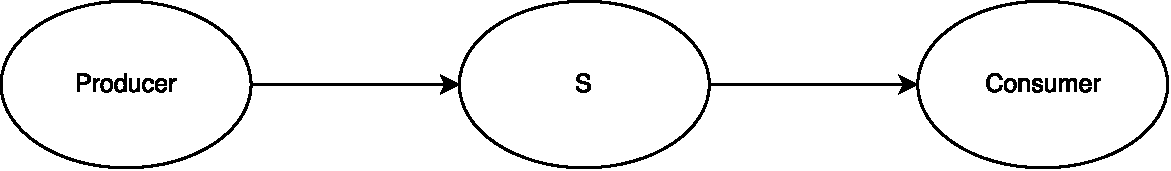
\includegraphics[scale=0.5]{images/app_model.pdf} 
\caption{An application model where a producer transmits data to a task A, which transforms the data, and sends the result to a consumer.}\label{fig:app_model}
\end{figure}

\subsection{Replication scheme}
In our framework, we ensure reliability based on task replication. We use active replication, where each replica receives the same input, and performs the same calculations. Figure~\ref{fig:app_model_replication} shows how the application looks like after replication of task $A$.

\begin{figure}[!hbt]
\centering
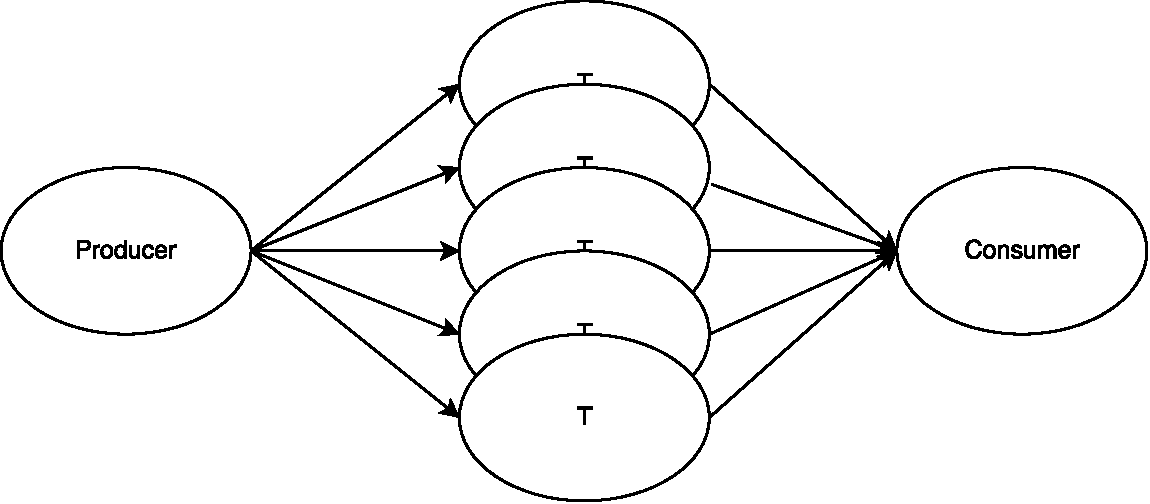
\includegraphics[scale=0.5]{images/app_model_replication.pdf} 
\caption{An application model where a producer transmits data to all replicas of task A, which transforms the data, and sends the result to a consumer.}\label{fig:app_model_replication}
\end{figure}

\subsection{Failure model}
In our framework, we assume the \emph{fail-stop} fault model. Nodes in the system have one of two states: \emph{running} or \emph{dead}. If a node dies, all running tasks on that node are dead. Furthermore, after a node has died, it will be restarted. However, the tasks that were being executed before it died will not be restarted when the node is restarted.

The reason for why a node died is irrelevant. Our model do not care whether a link died, or it was a hardware failure. 

We assume failures follow a Poission process, as this seems to be widely accepted in the research community. However, while most assumes constant failure rates, our failure distributions are dynamic and monitoring of the system resources and events allows for the framework to be self-adaptive and dynamic in terms of resource failure rates.

However, when a system first is put into action (use other words), no knowledge about the failure rates of the system is known. Therefore, when the system is set up, we to start with assume constant failure rates.

Furthermore, the time it takes to replicate a task is not known at deployment time. First when several applications has been deployed, and the time to replica tasks been measured, one can get an average replication time. The replication time will also be dynamic, and application dependent. Some tasks may take longer time to replicate than others, why a system wide average may be far from correct for a given application.


\subsection{Reliability model}
Conventionally, Mean-Time-To-Failure (MTTF) refers to non-repairable resources, while Mean-Time-Between-Failures (MTBF) refers to repairable objects \cite{effTaskReplMobGrid}. Since resources, e.g. computational nodes in the system, will be restarted upon failure, we use MTBF, defined as

\begin{equation} \label{eq:MTBF}
MTBF = (number\ of\ failures) / (total\ time)
\end{equation}

From equation~\ref{eq:MTBF} a reliability function can be expressed as 
\begin{equation} \label{eq:resource_reliability}
R_{r}(t) = e^{-t/MTBF_{r}}
\end{equation}

Equation~\ref{eq:resource_reliability} expresses the probability that a given resource will work for a time $t$.

For a complete analysis of system reliability, one must take all factors affecting reliability into account. However, including all factors if unfeasible.  \cite{factorsAffectingRel} lists 32 factors affecting the reliability of software, excluding environmental factors such as hardware and link failure. In our framework, we only care whether or not a node is available or has died.


Using replication of a task, and reliability defined as in definition~\ref{def:replica_reliability}, the probability that a task $T$  with $n$ replicas is successful during a time $t$ can be expressed as 

\begin{equation} \label{eq:task_reliability}
R_{T}(t) =  \prod\limits_{k=1}^n R_{Rep_k}(t)
\end{equation}

where $R_{Rep_k}(t)$ is the reliability that replica $k$ is reliable during the time $t$, which it takes to replicate an actor. Equation~\ref{eq:task_reliability} corresponds to definition~\ref{def:task_replica_reliability}, i.e. at least one replica is always running.

Assuming tasks themselves do not fail unless the resources they use fail, the reliability of a task replica is dependent on the reliability of the resources it uses. Limiting to model to node failure, either in terms of hardware failure or lost connectivity, equation~\ref{eq:task_reliability} can with equation~\ref{eq:resource_reliability} be re-written as

\begin{equation} \label{eq:task_reliability_2}
R_{T}(t) = \prod\limits_{k=1}^m  R_{Res_k}(t)
\end{equation}

Where $R_{Res_1}(t) \cdots R_{Res_m}(t)$ are the reliabilities of the $m$ resources on which the $n$ replicas are running. Using this model, reliability is only increased through replication if the replicas are scheduled on separate nodes.

Given a time $t$ it takes to replicate a task, a desired reliability level $\lambda$, and assuming the replicas are running on separate nodes, we get

\begin{equation} \label{eq:desired_rel}
\lambda \leq \prod\limits_{k=1}^n  R_{Res_k}(t)
\end{equation}

which must be fulfilled by the system. Since assuming hetereogenous failure rates for the various nodes, fulfilling equation~\ref{eq:desired_rel} is a scheduling problem.

The scheduling problem to fulfil a reliability $\lambda$ refers to selecting $n$ nodes on which to place $n$ replicas such as the reliability level of the task, expressed in equation~\ref{eq:task_reliability_2} exceeds $\lambda$.

\subsection{Self-adapting model}
%TODO

%TODO predict future MTBF? machine learning? cpu, memory usage, network load, etc.

\section{Implementation} \label{sec:implementation}
For implementing our model, we use an actor based application environment called \emph{Calvin} \cite{calvin}. Calvin is developed by \emph{Ericsson} and made open source in the summer of 2015. While Calvin is an application environment for IoT applications, is suites well for implementation of our model.

The Calvin framework consists of \emph{runtimes} on which one deploy applications consisting of connected \emph{actors}. We will use this model to reflect our system of nodes and application tasks. We will deploy a single runtime per node, and have an actor representing the task we will replicate.


\subsection{Scheduling algorithm}
A simple scheduling which fulfills equation~\ref{eq:desired_rel} is shown below:

\begin{algorithmic}
\State $n\gets 0$
\State $nodes\gets available\ nodes$\Comment{sorted by reliability, highest first}
\While {$\lambda \geq \prod\limits_{k=1}^n  R_{Res_k}(t)$}
	\State $node\gets nodes.pop$\Comment{take the node with highest reliability}
	\State{$replica\gets new\ replica$}
	\Call{place replica on node}{$replica$, $node$}
	\State $n\gets n + 1$
\EndWhile
\end{algorithmic}

\chapter{Evaluation} \label{ch:evaluation}
%TODO
performance metrics

\chapter{Limitations} \label{ch:limitations}

%TODO
Our model is obviously limited in that we do not account for link failures. However, the reliability model could easily be extended to include link failure probabilities, which then need to be taken into account in the scheduling algorihtm as well.

Furthermore, using a fail-stop fault model, we assume that when a node dies all other nodes are aware of this. This is clearly limiting, as in the case of a link failure, a node may become unavailable for one node while being availble for another.

Our definition of reliability excludes the possibility of tasks calculating incorrect results, which is the case when using a Byzantine fault model. Since already using active replication to ensure reliability, it would be trivial to extend it to use techniques such as majority voting or \emph{k-modular redundancy} in order to extend the reliability definition to also include that the job calculates the correct result.

Our primary objective is to ensure a certain level of reliability. By using active replication, we require a lot more resources, which puts an extra burden on the system. In addition, the extra load on the system may affect the execution time, thus decreasing task performance.

Our model is yet to be evaluated on highly unreliable system during extreme load. In this case, due to the unreliability of the system, the number of replicas needed to ensure the desired reliability level will increase. This will further increase the system load, thereby decreasing the reliability of the system even further. This may turn into a vicious circle.

\subsection{Reliability model}
\label{sec:limitations_reliability_model}
Many engineers and researchers base their reliability models on the assumption that components of a system fail in a statistically independent manner. This assumption is often violated in practice because environmental and system specific factors contribute to correlated failures, which can lower the reliability of a fault tolerant system. A simple method to quantify the impact of correlation on system reliability is needed to encourage models explicitly incorporating correlated failures. Previous approaches to model correlation are limited to systems consisting of two or three components or assume that the majority of the subsets of component failures are statistically independent. \cite{discContRelModel}


the interrelationship constraint between task modules has not been taken into account in calculation of distributed system reliability (DSR). In distributed simulation, the LPs simulation advances are bound by synchronization constraint, which will affect the executive time of system components. \cite{relModelDistSimSystem}

We do not take into account parameters such as X and Y [TODO].

Furthermore failure data which they have collected for their experiments through in-house testing cannot be compared with failures that can occur under actual operational environment \cite{surveyReliabilityDistr}

A lot of researchers are of the view that service providers must provide some other detail to compute reliability of both type of services i.e. atomic service and composite service. Such as, external services it uses, how service are glued together in composite service, how frequently they call each other, and flow graph describing behavior of service [2]. Service Oriented Reliability Model (SORM) [18] computed reliability of atomic and composite services exploiting distinct technique \cite{surveyReliabilityDistr}

Given the failure probability Pfik of each one of the mi replicas Ti k of task Ti , the new failure probability P fi0 for task Ti is:
0 mi Y
Pfi =Pfi· Pfik. (2) k=1
The above corresponds to the probability of the event “all the replicas and the original task fail”. Respectively, the success probability is equal to the probability of the event “the original task or at least one of its replicas executes successfully”. The number of replicas issued depends on the failure probabilities of the original tasks and on the desired fault tolerance level in the Grid infrastructure.  \cite{effTaskReplMobGrid}


\chapter{Future Work} \label{ch:future_work}
%TODO
Replication impose extra buden on the system as additional resources are needed and computational power is wasted. By combining checkpointing techniques with active replication, the number of replicas needed could possible be decreased. (\cite{adaptiveCheckPointAndRep} combines checkpointing and replication)
\\\\
Predict future failures - machine learning (many parameters could be taken into account), and when the probability of failure reaches above a certain threshold, the running tasks on that node could be migrated. A high reliability in failure prediction allows for fewer replicas to be needed.

\subsection{Extended model}
Reliability of server’s availability and scalability (such as File Server, DB servers, Web servers, and email servers, etc.), communication infrastructure, and connecting devices. \cite{surveyReliabilityDistr}

For measure reliability according to the dynamic definition (Definition \ref{def:dyn_reliability}) we will use the following formula:

\begin{equation} \label{eq:overall_reliability}
R(t) = R_{1}(t) \cdot R_{2}(t) \cdots R_{n}(t)
\end{equation}
where $R_{k}(t)$ is the probability that factor $k$ is free from failures during time $t$. Some factors to consider are software (the program itself), OS (the device executing the program), hardware, network, electrical supply and load. The factors can be divided into static and dynamic factors. The static factors are those which does not change that frequently, such as electrical supply or hardware/software while the dynamic factors are those changing more frequently, for instance the current load (or load average for last 5 minutes etc). For simplicity we will use one reliability for all static factors and chose a number of dynamic factors to consider.


\chapter{Conclusions} \label{ch:conclusions}

\begin{thebibliography}{50}

\bibitem{taskAllocation}
	Sol M. Shatz, Jia-Ping Wang and Masanori Goto,
	\emph{Task Allocation for Maximizing Reliability of Distributed Computer Systems},
	Computers, IEEE Transactions on, Volume 41  Issue 9,
	Sep 1992
	
\bibitem{surveyReliabilityDistr}
	Waseem Ahmed and Yong Wei Wu,
	\emph{A survey on reliability in distributed systems},
	Journal of Computer and System Sciences Volume 78 Issue 8,
	December 2013, Pages 1243–1255

\bibitem{compStudyLoadAndCloud}
	Mayanka Katyal and Atul Mishra,
	\emph{A Comparative Study of Load Balancing Algorithms in Cloud Computing Environmen},
	International Journal of Distributed and Cloud Computing, Volume 1 Issue 2,
	2013

\bibitem{surveyFaultParallel}
	Michael Treaster,
	\emph{A Survey of Fault-Tolerance and Fault-Recovery Techniques in Parallel Systems},
	Cornell University Library,
	Jan 2005

\bibitem{gridWorkflow}
	Soonwook Hwang and Carl Kesselman,
	\emph{Grid Workflow: A Flexible Failure Handling Framework for the Grid},
	High Performance Distributed Computing, 2003. Proceedings. 12th IEEE International Symposium on, p. 	126-137, 
	June 2003

\bibitem{perfAnalysisLoadCloud}
	Prashant D. Maheta , Kunjal Garala and Namrata Goswami,
	\emph{A Performance Analysis of Load Balancing Algorithms in Cloud Environment},
	Computer Communication and Informatics (ICCCI), 2015 International Conference on,
	Jan 2015
	
\bibitem{taskSchedulingReplication}
	Shuli Wang et. al.
	\emph{A Task Scheduling Algorithm Based on Replication for Maximizing Reliability on Heterogeneous Computing Systems},
	Parallel \& Distributed Processing Symposium Workshops (IPDPSW), 2014 IEEE International, p. 1562 1571, 
	May 2014

\bibitem{softRelRoadmap}
	Michael R. Lyu
	\emph{Reliability Engineering: A Roadmap},
	Future of Software Engineering, FOSE ’07, p. 153-170,
	23–25 May 2007
	
\bibitem{dynAdaptRepl}
	Guessoum Z. et. al.
	\emph{Dynamic and Adaptive Replication for Large-Scale Reliable Multi-agent Systems},
	Lecture Notes in Computer Science pp 182-198,
	April 2003

\bibitem{algoMaxRelEndToEndConstraint}
Distributed workflow mapping algorithm for maximized reliability under end-to-end delay constraint

\bibitem{algoMinExTime}
Matching and Scheduling Algorithms for Minimising Execution Time and Failure Probability of Applications in Heterogeneous Computing

\bibitem{relModelDistSimSystem}
Reliability model of distributed simulation system

\bibitem{optTaskAllocationForMaxRel}
Optimal task allocation for maximizing reliability in distributed real-time systems

\bibitem{perfImplPerCheckPoint}
Performance Implications of Periodic Checkpointing on Large-scale Cluster Systems

\bibitem{studyOfFailures}
A large-scale study of failures in high-performance computing systems

\bibitem{discContRelModel}
Discrete and continuous reliability models for systems with identically distributed correlated components

\bibitem{effTaskReplMobGrid}
	Antonios Litke et. al.,	
	\emph{Efficient task replication and management for adaptive fault tolerance in Mobile Grid environments},
	Future Generation Computer Systems Vol 23 Issue 2 p. 163-178,
	February 2007

\bibitem{realTimeSchedAlgo}
Real-time fault-tolerant scheduling algorithm for distributed computing systems

\bibitem{distDiagnosis}
Distributed Diagnosis in Dynamic Fault Environments

\bibitem{optCheckpointInterval}
A higher order estimate of the optimum checkpoint interval for restart dumps

\bibitem{factorsAffectingRel}
An analysis of factors affecting software reliability

\bibitem{SLASched}
SLA-aware Resource Scheduling for Cloud Storage

\bibitem{algoOptTimeMaxRel}
An Algorithm for Optimized Time, Cost, and Reliability in a Distributed Computing System

\bibitem{imprRelAdaptRL}
Improving reliability in resource management through adaptive reinforcement learning for distributed systems

\bibitem{selfAdaptRel}
Self-Adapting Reliability in Distributed Software Systems

\bibitem{schedReplicas}
Scheduling Fault-Tolerant Distributed Hard Real-Time Tasks Independently of the Replication Strategies

\bibitem{calvin}
Calvin - Merging Cloud and IoT

\bibitem{taskAllocationSwarm}
Task allocation for maximizing reliability of a distributed system using hybrid particle swarm optimization

\bibitem{optResourceAllMaxPerformance}
Optimal Resource Allocation for Maximizing Performance and Reliability in Tree-Structured Grid Services 

\bibitem{matchSchedAlgoMinFailure}
Matching and Scheduling Algorithms for Minimizing Execution Time and Failure Probability of Applications in Heterogeneous Computing

\bibitem{safetyRelTaskAllocation}
Safety and Reliability Driven Task Allocation in Distributed Systems

\bibitem{improvedTaskAllMaxRel}
Improved Task-Allocation Algorithms to Maximize Reliability of Redundant Distributed Computing Systems 

\bibitem{designFaultTolerantSched}
Design of a Fault-Tolerant Scheduling System for Grid Computing

\bibitem{evalReplicationSched}
Evaluation of replication and rescheduling heuristics for grid systems with varying resource availability

\bibitem{faultTolerantSchedPolicy}
Fault-Tolerant Scheduling Policy for Grid Computing Systems

\bibitem{adaptiveCheckPointAndRep}
Adaptive Task Checkpointing and Replication: Toward Efficient Fault-Tolerant Grids

\end{thebibliography}

\begin{appendices}
\chapter{A}

\end{appendices}











% Below is the report template found online

\chapter[Short on Formatting]{Formatting}
Avoid empty spaces between \textit{chapter}-\textit{section}, \textit{section}-\textit{sub-section}. For instance, a very brief summary of the chapter would be one way of bridging the chapter heading and the first section of that chapter.
\section{Page Size and Margins}
Use A4 paper, with the text margins given in Table \ref{tab:margins}.
\begin{table}[!hbt]
\centering
\caption{Text margins for A4.}\label{tab:margins}
\begin{tabular}{cc}
\hline
\textbf{margin} & \textbf{space} \\
\hline 
top &  3.0cm\\ 

bottom & 3.0cm \\ 
 
left (inside) & 2.5cm \\ 

right (outside) & 2.5cm \\ 

binding offset & 1.0cm \\ 
\hline 
\end{tabular} 
\end{table}

\section{Typeface and Font Sizes}
The fonts to use for the reports are \textbf{TeX Gyre Termes} (a \textbf{Times New Roman} clone) for serif fonts, \textsf{\textbf{TeX Gyre Heros}} (a \textsf{\textbf{Helvetica}} clone) for sans-serif fonts, and finally \texttt{\textbf{TeX Gyre Cursor}} (a \texttt{\textbf{Courier}} clone) as mono-space font. All these fonts are included with the TeXLive 2013 installation. Table \ref{tab:fonts} lists the most important text elements and the associated fonts.
\begin{table}[!hbt]
\caption{Font types, faces and sizes to be used.}\label{tab:fonts}

 \begin{tabular}{ l c c c}
\hline 
\textbf{Element} & \textbf{Face} & \textbf{Size}  & \textbf{\LaTeX size}  \\ 
\hline 
{\huge \textbf{Ch. label}} & {\huge \textbf{serif, bold}} & \thefontsize\huge & \verb+\huge+ \\ 
{\Huge \textbf{Chapter}} & {\Huge \textbf{serif, bold}} & \thefontsize\Huge & \verb+\Huge+ \\ 
{\LARGE \textsf{\textbf{Section}}} & {\Large \textsf{\textbf{sans-serif, bold}}} & \thefontsize\LARGE &  \verb+\LARGE+  \\ 
{\Large \textsf{\textbf{Subsection}}} & {\Large \textsf{\textbf{sans-serif, bold}}} & \thefontsize\Large & \verb+\Large+ \\ 
{\large \textsf{\textbf{Subsubsection}}} & {\Large \textsf{\textbf{sans-serif, bold}}} & \thefontsize\large &  \verb+\large+ \\ 
Body & serif & \thefontsize\normalsize & {\footnotesize \verb+\normalsize+} \\
%{\footnotesize Footnote} & serif  & \thefontsize\footnotesize & {\footnotesize \verb+\footnotesize+} \\
{\footnotesize \textsc{Header}} & {\footnotesize \textsc{serif, SmallCaps}} & \thefontsize\footnotesize &  \\
Footer (page numbers) & serif, regular & \thefontsize\normalsize &  \\
\hline
\textbf{Figure label} & \textbf{serif, bold} & \thefontsize\normalsize & \\
Figure caption & serif, regular & \thefontsize\normalsize & \\
\textsf{In figure} & \textsf{sans-serif} & \textit{any} & \\
\textbf{Table label} & \textbf{serif, bold} & \thefontsize\normalsize & \\
Table caption and text & serif, regular & \thefontsize\normalsize & \\
\texttt{Listings} & \texttt{mono-space} & $\le$ \thefontsize\normalsize & \\
\hline 
\end{tabular} 
\end{table}

\subsection{Headers and Footers}
Note that the page headers are aligned towards the outside of the page (right on the right-hand page, left on the left-hand page) and they contain the section title on the right and the chapter title on the left respectively, in \textsc{SmallCaps}. The footers contain only page numbers on the exterior of the page, aligned right or left depending on the page. The lines used to delimit the headers and footers from the rest of the page are $0.4 pt$ thick, and are as long as the text.

\subsection{Chapters, Sections, Paragraphs}
Chapter, section, subsection, etc. names are all left aligned, and numbered as in this document. 

Chapters always start on the right-hand page, with the label and title separated from the rest of the text by a $0.4 pt$ thick line.

Paragraphs are justified (left and right), using single line spacing. Note that the first paragraph of a chapter, section, etc. is not indented, while the following are indented.

\subsection{Tables}
Table captions should be located above the table, justified, and spaced 2.0cm from left and right (important for very long captions). Tables should be numbered, but the numbering is up to you, and could be, for instance:
\begin{itemize}
\item \textbf{Table X.Y} where X is the chapter number and Y is the table number within that chapter. (This is the default in \LaTeX. More on {\LaTeX} can be found on-line, including whole books, such as \cite{goossens93}.) or
\item \textbf{Table Y} where Y is the table number within the whole report
\end{itemize}
As a recommendation, use regular paragraph text in the tables, bold headings and avoid vertical lines (see Table \ref{tab:fonts}). 

\subsection{Figures}
Figure labels, numbering, and captions should be formed similarly to tables. As a recommendation, use vector graphics in figures (Figure \ref{fig:vectorg}), rather than bitmaps (Figure \ref{fig:rasterg}). Text within figures usually looks better with sans-serif fonts.
\begin{figure}[!hbt]
\centering

\includegraphics[scale=2.5]{images/examplepic1.pdf} 
\caption{A PDF vector graphics figure. Notice the numbering and placement of the caption. The caption text is indented 2.0cm from both left and right text margin.}\label{fig:vectorg}
\end{figure}

\begin{figure}[!hbt]
\centering

\includegraphics[scale=2.5]{images/examplepic3.jpg} 
\caption{A JPEG bitmap figure. Notice the bad quality of such an image when scaling it. Sometimes bitmap images are unavoidable, such as for screen dumps.}\label{fig:rasterg}
\end{figure}
For those interested in delving deeper into the design of graphical information display, please refer to books such as \cite{Tufte:1986, few2012show}.

\section{Mathematical Formulae and Equations}
You are free to use in-text equations and formulae, usually in \textit{italic serif} font. For instance: $S = \sum_i a_i$. We recommend using numbered equations when you do need to refer to the specific equations:
\begin{equation}
E = \int_0^{\delta} P(t) dt \quad \longleftrightarrow \quad E = m c^2
\end{equation}
The numbering system for equations should be similar to that used for tables and figures.

\section{References}
Your references should be gathered in a \textbf{References} section, located at the end of the document (before \textbf{Appendices}). We recommend using number style references, ordered as appearing in the document or alphabetically. Have a look at the references in this template in order to figure out the style, fonts and fields. Web references are acceptable (with restraint) as long as you specify the date you accessed the given link \cite{fontspec, CTAN}. You may of course use URLs directly in the document, using mono-space font, i.e. \url{http://cs.lth.se/}.

\section{Colours}
As a general rule, all theses are printed in black-and-white, with the exception of selected parts in selected theses that need to display colour images essential to describing the thesis outcome (\textit{computer graphics}, for instance).

A strong requirement is for using \textbf{black text on white background} in your document's main text. Otherwise we do encourage using colours in your figures, or other elements (i.e. the colour marking internal and external references) that would make the document more readable on screen. You may also emphasize table rows, columns, cells, or headers using white text on black background, or black text on light grey background.

Finally, note that the document should look good in black-and-white print. Colours are often rendered using monochrome textures in print, which makes them look different from on screen versions. This means that you should choose your colours wisely, and even opt for black-and-white textures when the distinction between colours is hard to make in print. The best way to check how your document looks, is to print out a copy yourself.

\chapter{Language}

You are strongly encouraged to write your report in English, for two reasons. First, it will improve your use of English language. Second, it will increase visibility for you, the author, as well as for the Department of Computer Science, and for your host company (if any).

However, note that your examiner (and supervisors) are not there to provide you with extensive language feedback. We recommend that you check the language used in your report in several ways:
\begin{description}
\item[Reference books] dedicated to language issues can be very useful. \cite{heffernan2000writing} 
\item[Spelling and grammar checkers] which are usually available in the commonly used text editing environments.
\item[Colleagues and friends] willing to provide feedback your writing.
\item[Studieverkstaden] is a university level workshop, that can help you with language related problems (see \href{http://www.lu.se/studera/livet-som-student/service-och-stod/studieverkstaden}{Studieverkstaden}'s web page).
\item[Websites] useful for detecting language errors or strange expressions, such as
\begin{itemize}
\item \url{http://translate.google.com}
\item \url{http://www.gingersoftware.com/grammarcheck/}
\end{itemize}
\end{description}

\section{Style Elements}
Next, we will just give some rough guidelines for good style in a report written in English. Your supervisor and examiner as well as the aforementioned \textbf{Studieverkstad} might have a different  take on these, so we recommend you follow their advice whenever in doubt. If you want a reference to a short style guide, have a look at \cite{shortstyleguide}.

\subsubsection{Widows and Orphans}

Avoid \textit{widows} and \textit{orphans}, namely words or short lines at the beginning or end of a paragraph, which are left dangling at the top or bottom of a column, separated from the rest of the paragraph.

\subsubsection{Footnotes}

We strongly recommend you avoid footnotes. To quote from \cite{OGSW}, \textit{Footnotes are frequently misused by containing information which should either be placed in the text or excluded altogether. They should be avoided as a general rule and are acceptable only in exceptional cases when incorporation of their content in the text  [is] not possible.} 

\subsubsection{Active vs. Passive Voice}

Generally active voice (\textit{I ate this apple.}) is easier to understand than passive voice (\textit{This apple has been eaten (by me).}) In passive voice sentences the actor carrying out the action is often forgotten, which makes the reader wonder who actually performed the action. In a report is important to be clear about who carried out the work. Therefore we recommend to use active voice, and preferably the plural form \textit{we} instead of \textit{I} (even in single author reports).

\subsubsection{Long and Short Sentences}
A nice brief list of sentence problems and solutions is given in \cite{yalesentences}. Using choppy sentences (too short) is a common problem of many students. The opposite, using too long sentences, occurs less often, in our experience.

\subsubsection{Subject-Predicate Agreement}
A common problem of native Swedish speakers is getting the subject-predicate (verb) agreement right in sentences. Note that a verb must agree in person and number with its subject. As a rough tip, if you have subject ending in \textit{s} (plural), the predicate should not, and the other way around. Hence, \textit{only one s}. Examples follow:
\begin{description}
\item[incorrect] He have to take this road.
\item[correct] He has to take this road.
\end{description}
\begin{description}
\item[incorrect] These words forms a sentence.
\item[correct] These words form a sentence.
\end{description}
\noindent In more complex sentences, getting the agreement right is trickier. A brief guide is given in  the \textit{20 Rules of Subject Verb Agreement} \cite{subjectverb}.

\chapter{Structure}
It is a good idea to discuss the structure of the report with your supervisor rather early in your writing. Given next is a generic structure that is a starting point, but by no means the absolute standard. Your supervisor should provide a better structure for the specific field you are writing your thesis in. Note also that the naming of the chapters is not compulsory, but may be a helpful guideline.
\begin{description}
\item[Introduction] should give the background of your work. Important parts to cover:
\begin{itemize}
\item Give the context of your work, have a short introduction to the area.
\item Define the problem you are solving (or trying to solve).
\item Specify your contributions. What does this particular work/report bring to the research are or to the body of knowledge? How is the work divided between the co-authors? (This part is essential to pinpoint individual work. For theses with two authors, it is compulsory to identify which author has contributed with which part, both with respect to the work and the report.)
\item Describe related work (literature study). Besides listing other work in the area, mention how is it related or relevant to your work. The tradition in some research area is to place this part at the end of the report (check with your supervisor).
\end{itemize}
\item[Approach] should contain a description of your solution(s), with all the theoretical background needed. On occasion this is replaced by a subset or all of the following:
\begin{itemize}
\item \textbf{Method}: describe how you go about solving the problem you defined. Also how do you show/prove that your solution actually works, and how well does it work.
\item \textbf{Theory}: should contain the theoretical background needed to understand your work, if necessary.
\item \textbf{Implementation}: if your work involved building an artefact/implementation, give the details here. Note, that this should not, as a rule, be a chronological description of your efforts, but a view of the result. There is a place for insights and lamentation later on in the report, in the Discussion section.
\end{itemize}
\item[Evaluation] is the part where you present the finds. Depending on the area this part contains a subset or all of the following: 
\begin{itemize}
\item \textbf{Experimental Setup} should describe the details of the method used to evaluate your solution(s)/approach. Sometimes this is already addressed in the \textbf{Method}, sometimes this part replaces \textbf{Method}.
\item \textbf{Results} contains the data (as tables, graphs) obtained via experiments  (benchmarking, polls, interviews).
\item \textbf{Discussion} allows for a longer discussion and interpretation of the results from the evaluation, including extrapolations and/or expected impact. This might also be a good place to describe your positive and negative experiences related to the work you carried out.
\end{itemize} 
Occasionally these sections are intermingled, if this allows for a better presentation of your work. However, try to distinguish between measurements or hard data (results) and extrapolations, interpretations, or speculations (discussion).
\item[Conclusions] should summarize your findings and possible improvements or recommendations.
\item[Bibliography] is a must in a scientific report. {\LaTeX} and \texttt{bibtex} offer great support for  handling references and automatically generating bibliographies.
\item[Appendices] should contain lengthy details of the experimental setup, mathematical proofs, code download information, and shorter code snippets. Avoid longer code listings. Source code should rather be made available for download on a website or on-line repository of your choosing.

\end{description}
\makebibliography{MyMSc}

\begin{appendices}
\chapter{About This Document}
The following environments and tools were used to create this document:
\begin{itemize}
\item operating system: Mac OS X 10.10.1
\item tex distribution: MacTeX-2014, \url{http://www.tug.org/mactex/}
\item tex editor: Texmaker 4.4.1 for Mac, \url{http://www.xm1math.net/texmaker/} for its XeLaTeX flow (recommended) or pdfLaTeX flow
\item bibtex editor: BibDesk 1.6.3 for Mac, \url{http://bibdesk.sourceforge.net/}
\item fonts \texttt{cslthse-msc.cls} document class): 
\begin{description}
\item{for XeLaTeX}: TeX Gyre Termes, \textsf{TeX Gyre Heros}, \texttt{TeX Gyre Cursor} (installed from the TeXLive 2013)
\item{for pdfLaTeX}: TeX Gyre font packages: tgtermes.sty, tgheros.sty, tgcursor.sty, gtxmath.sty (available through TeXLive 2013) 
\end{description} 
\item picture editor: OmniGraffle Professional 5.4.2
\end{itemize}

\noindent A list of the essential \LaTeX packages needed to compile this document follows (all except \texttt{hyperref} are included in the document class):
\begin{itemize}
\item \texttt{fontspec}, to access local fonts, needs the XeLaTeX flow
\item \texttt{geometry}, for page layout
\item \texttt{titling}, for formatting the title page
\item \texttt{fancyhdr}, for custom headers and footers
\item \texttt{abstract}, for customizing the abstract
\item \texttt{titlesec}, for custom chapters, sections, etc.
\item \texttt{caption}, for custom tables and figure captions
\item \texttt{hyperref}, for producing PDF with hyperlinks
\item \texttt{appendix}, for appendices
\item \texttt{printlen}, for printing text sizes
\item \texttt{textcomp}, for text companion fonts (e.g. bullet)
\end{itemize}

\noindent Other useful packages:
\begin{itemize}
\item \texttt{listings}, for producing code listings with syntax colouring and line numbers
\end{itemize}

\chapter{List of Changes}
\subsubsection{Since 2015/04/27}
\begin{itemize}
\item Improved the \textbf{Structure} chapter and added more detailed comments for each part.
\end{itemize}

\subsubsection{Since 2014/02/18}
\begin{itemize}
\item Added the possibility to specify two supervisors. Use either of the \verb+\supervisor{}+ or \verb+\supervisors{}{}+ commands to set the names and contacts on the first page.
\end{itemize}

\subsubsection{Since 2013/09/23}
\begin{itemize}
\item Added missing colon ":" after \textit{Examiner} on the front page. 
\end{itemize}

\subsubsection{Since 2013/08/30}
\begin{itemize}
\item Changed fonts from Garamond (Times New Roman), Helvetica (Arial), Courier (Source Code Pro) to Tex Gyre fonts, namely Termes, Heros, Cursor, which are freely available with TexLive 2013 installation. These are all clones of Times New Roman, Helvetica and Courier, respectively. Garamond is problematic on some systems, being a non-freely available font.
\item Corrected the \textit{Face} column in Table \ref{tab:fonts} to correctly depict the font face.
\end{itemize}

\subsubsection{Since 2013/02/22}
\begin{itemize}
\item Number of words required in the abstract changed to 150 (from 300).
\end{itemize}

\subsubsection{Since 2013/02/15}
\begin{itemize}
\item Made a separate document class, for clarity.
\item made it work with pdfLaTeX and garamond.sty, in addition to XeLaTeX and true type fonts. It is up to the user to get the hold of the garamond.zip from \url{http://gael-varoquaux.info/computers/garamond/index.html}.
\end{itemize}
\end{appendices}


\end{document}
